\documentclass[a4paper, 12pt]{article} % Uses article class in A4 format

%----------------------------------------------------------------------------------------
%	FORMATTING
%----------------------------------------------------------------------------------------

\addtolength{\hoffset}{-2.25cm}
\addtolength{\textwidth}{4.5cm}
\addtolength{\voffset}{-3.25cm}
\addtolength{\textheight}{5cm}
\setlength{\parskip}{0pt}
\setlength{\parindent}{0in}

%----------------------------------------------------------------------------------------
%	PACKAGES AND OTHER DOCUMENT CONFIGURATIONS
%----------------------------------------------------------------------------------------
\usepackage{tabularx}
\usepackage[runin]{abstract}
\usepackage{charter} % Use the Charter font
\usepackage[utf8]{inputenc} % Use UTF-8 encoding
\usepackage{microtype} % Slightly tweak font spacing for aesthetics

\usepackage[english]{babel} % Language hyphenation and typographical rules

\usepackage{amsthm, amsmath, amssymb} % Mathematical typesetting
\usepackage{float} % Improved interface for floating objects
\usepackage[final, colorlinks = true, 
            linkcolor = black, 
            citecolor = black]{hyperref} % For hyperlinks in the PDF
\usepackage{graphicx, multicol} % Enhanced support for graphics
\graphicspath{{Figure/}{logo/}}
\usepackage{color}
\usepackage{xcolor} % Driver-independent color extensions
\usepackage{marvosym, wasysym} % More symbols
\usepackage{rotating} % Rotation tools
\usepackage{censor} % Facilities for controlling restricted text
\usepackage{listings, lstautogobble} % Environment for non-formatted code
\usepackage{pseudocode} % Environment for specifying algorithms in a natural way
\usepackage{algorithm}
\usepackage{algpseudocode}
\renewcommand{\algorithmicrequire}{\textbf{Input:}}
\renewcommand{\algorithmicensure}{\textbf{Output:}}
\usepackage{booktabs} % Enhances quality of tables

\usepackage{cases}
\usepackage{bookmark}

\usepackage{tikz-qtree} % Easy tree drawing tool
\tikzset{every tree node/.style={align=center,anchor=north},
         level distance=2cm} % Configuration for q-trees

\usepackage[backend=biber,style=numeric,
            sorting=nyt]{biblatex} % Complete reimplementation of bibliographic facilities

\usepackage{csquotes} % Context sensitive quotation facilities

\usepackage[yyyymmdd]{datetime} % Uses YEAR-MONTH-DAY format for dates
\renewcommand{\dateseparator}{-} % Sets dateseparator to '-'

\usepackage{fancyhdr} % Headers and footers
\pagestyle{fancy} % All pages have headers and footers
\fancyhead{}\renewcommand{\headrulewidth}{0pt} % Blank out the default header
\fancyfoot[L]{} % Custom footer text
\fancyfoot[C]{} % Custom footer text
\fancyfoot[R]{\thepage} % Custom footer text

\newcommand{\note}[1]{\marginpar{\scriptsize \textcolor{red}{#1}}} % Enables comments in red on margin

\usepackage{fontspec}
\setmonofont{Consolas}
\definecolor{codegreen}{rgb}{0,0.6,0}
\definecolor{codegray}{rgb}{0.5,0.5,0.5}
\definecolor{codemauve}{rgb}{0.58,0,0.82}

\lstset{ %
	language=python,                % choose the language of the code
	basicstyle=\footnotesize\ttfamily,       % the size of the fonts that are used for the code
	numbers=left,                   % where to put the line-numbers
	numberstyle=\tiny\color{codegray},      % the size of the fonts that are used for the line-numbers
	stepnumber=1,                   % the step between two line-numbers. If it is 1 each line will be numbered
	numbersep=5pt,                  % how far the line-numbers are from the code
	backgroundcolor=\color{white},  % choose the background color. You must add \usepackage{color}
	showspaces=false,               % show spaces adding particular underscores
	showstringspaces=false,         % underline spaces within strings
	showtabs=false,                 % show tabs within strings adding particular underscores
	frame=single,                   % adds a frame around the code
	tabsize=4,                      % sets default tabsize to 4 spaces  
	captionpos=b,                   % sets the caption-position to bottom
	breaklines=true,                % sets automatic line breaking
	breakatwhitespace=false,        % sets if automatic breaks should only happen at whitespace
	escapeinside={\%*}{*)},
	commentstyle=\color{codegreen},
	keywordstyle=\bfseries\color{magenta},
	stringstyle=\color{red},
	identifierstyle=\color{codemauve},
	keepspaces=true
	autogobble=true
}

%----------------------------------------------------------------------------------------

\begin{document}

%----------------------------------------------------------------------------------------
%	TITLE SECTION
%----------------------------------------------------------------------------------------

\title{Template} % Article title
\fancyhead[C]{}
\hrule \medskip % Upper rule
\begin{minipage}{0.295\textwidth} % Left side of title section
    \raggedright
    DATA130008\\ % Your course code
    \footnotesize % Authors text size
    \hfill\\
    Artificial Intelligence\\ % Your course name
\end{minipage}
\begin{minipage}{0.4\textwidth} % Center of title section
    \centering
    \large % Title text size
    Midterm 1 Report\\ % Assignment title and number
    \normalsize % Subtitle text size
    Gomoku AI With Alpha-Beta Pruning\\ % Assignment subtitle
\end{minipage}
\begin{minipage}{0.295\textwidth} % Right side of title section
    \raggedleft
    BoYuan Yao 19307110202\\ % Your name
    LeiRu Long 19307130350
    \footnotesize % Email text size
\end{minipage}
\medskip\hrule % Lower rule
\bigskip

%----------------------------------------------------------------------------------------
%	ARTICLE CONTENTS
%----------------------------------------------------------------------------------------


%----------------------------------------------------------------------------------------
\begin{multicols}{2}
    [
        \section{Introduction}
    ]
    A game is a zero-sum game in which two players take turns, with complete information and certainty. Gomoku is such a two-player strategical board game. The freest rule of Gomoku is that during the game, both sides take turns to place a black or white piece on the board, and the first to achieve five or more consecutive pieces of the same color in the horizontal, vertical or diagonal direction wins.
    
    Although it seems that there are various moves in Gomoku, since Gomoku is a complete information zero-sum game, each move can be expanded out into a huge game tree. In this game tree, the score of each node represents how bad the situation is for the player, and the two adjacent layers are player actions and enemy actions respectively. When the player moves, he chooses the node with the highest score, and when the enemy moves, he chooses the node with the lowest score, which is the most disadvantageous to the player. Thus, we can create an AI for Gomoku based on the alpha-beta algorithm.
    
    To make the alpha-beta algorithm available, we must first figure out the way to evaluate situations on the board, as described in Section 2. Besides, considering exponential time cost, techniques are applied to make a well-performed AI in following section. In Section 4, we show experimental results against other AI. In the end, we point out several work to do in the future for further improvement.
        
\end{multicols}


%----------------------------------------------------------------------------------------
\begin{multicols}{2}
  [
      \section{Alpha-beta Algorithm}
      For the sake of unity of expression, we assume that the AI plays black and the opponent plays white.
  ]
  \subsection{Evaluation}
  In the ideal alpha-beta pruning algorithm, agent should search as deep as possible, which means if could reach leaf nodes where one side of the game win. But in real life, we are not capable to do it due to the exponential complexity of the tree search. Therefore, an excellent proximal evaluation is a key factor to the success of alpha-beta pruning algorithm. Here we design the evaluation strategy as follows.
  
  \subsubsection{Score For Each Pattern}
  We summarize the basic patterns of the pieces in Gomoku and assign scores to different patterns in table1. As for the name of patterns' names, the N refers to the sequence that can be added one move to become N+1, while the BLOCK\_N refers to a sequence that only can become BLOCK\_(N+1) with one specific move.
    \begin{table}[H]
    \setlength\tabcolsep{3pt}
    \begin{center}
    	\scalebox{0.8}{
      	\begin{tabularx}{10cm}{ccc}
			\toprule
        	\textbf{Pattern Type} & \textbf{Definition} & \textbf{Value}\\
        	\midrule
        	FIVE 
        	&\begin{minipage}[b]{0.3\columnwidth}
		    	\centering
		    	\raisebox{-.5\height}{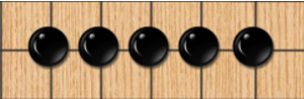
\includegraphics[width=\linewidth]{five.png}}
	      	\end{minipage}
	      	& 10000000 \\
        	\midrule
       		FOUR & \begin{minipage}[b]{ 0.3\columnwidth}
		   	\centering
		   	\raisebox{-.5\height}{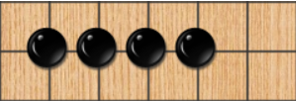
\includegraphics[width=\linewidth]{4.png}}
	     	\end{minipage} & 100000 \\
       		\midrule
       		BLOCKED\_FOUR & \begin{minipage}[b]{ 0.3\columnwidth}
		   	\centering
		   	\raisebox{-.5\height}{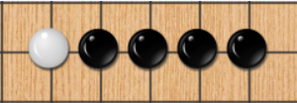
\includegraphics[width=\linewidth]{b4.png}}
	     	\end{minipage} & 10000 \\
      		\midrule
      		THREE & \begin{minipage}[b]{ 0.3\columnwidth}
		   		\centering
		   		\raisebox{-.5\height}{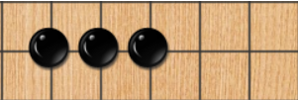
\includegraphics[width=\linewidth]{3.png}}
	     	\end{minipage} & 1000 \\
      		\midrule
     		BLOCKED\_THREE & \begin{minipage}[b]{ 0.3\columnwidth}
		   		\centering
		   		\raisebox{-.5\height}{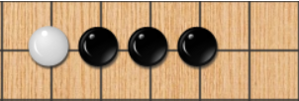
\includegraphics[width=\linewidth]{b3.png}}
	     	\end{minipage} & 100 \\
      		\midrule
      		TWO &\begin{minipage}[b]{ 0.3\columnwidth}
		   		\centering
		   		\raisebox{-.5\height}{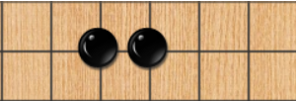
\includegraphics[width=\linewidth]{2.png}}
	     	\end{minipage} & 100 \\
    		\midrule
      		BLOCKED\_TWO & \begin{minipage}[b]{ 0.3\columnwidth}
		   		\centering
		   		\raisebox{-.5\height}{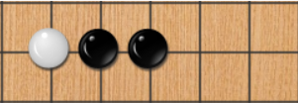
\includegraphics[width=\linewidth]{b2.png}}
	     	\end{minipage} & 10 \\
      		\midrule
      		ONE & \begin{minipage}[b]{ 0.3\columnwidth}
		   		\centering
		   		\raisebox{-.5\height}{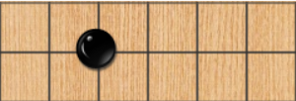
\includegraphics[width=\linewidth]{1.png}}
	     		\end{minipage} & 10 \\
      		\midrule
      		BLOCKED\_ONE & \begin{minipage}[b]{ 0.3\columnwidth}
		   		\centering
		   		\raisebox{-.5\height}{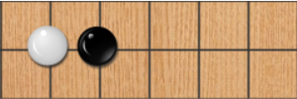
\includegraphics[width=\linewidth]{b1.png}}
	     	\end{minipage} & 1 \\
    	\bottomrule
	\end{tabularx}
}
  	\caption{Score For Each Pattern}
	\label{tab:table1}
\end{center}
\end{table}

    \subsubsection{Point Evaluation}
    The score of a move is evaluated based on how well it attack and how much it weaken the opponent. Here We divide dots into two categories, empty points and colored points.
    
    For assigning a value to a colored point, we use the radius of 6 grid, scan its horizontal(h), vertical(v), and diagonal directions(d1/d2). Calculate patterns with the same color formed in each direction respectively, and take the largest in that direction. Finally, sum up the scores in the four directions to get a colored point score.
    
    For assigning a value to a empty point, we assume it's black and white and calculate the score respectively. Thus it has a positive white score for the enemy and black score for AI player.
    \begin{figure}[H]
    \centering
    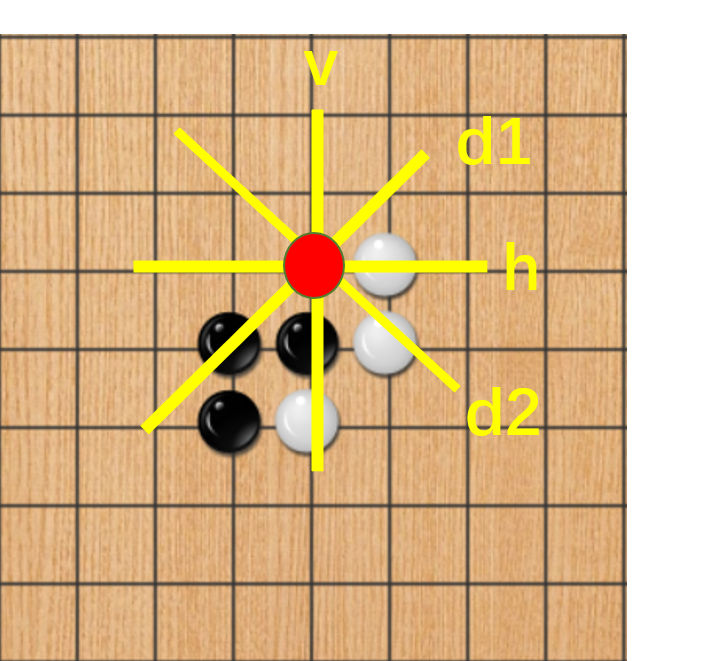
\includegraphics[scale=0.4]{example.png}
    \caption{An example of evaluating a empty point }
    \label{figure}
    \end{figure}
    In this example the white score of red point is:
    $$
    \begin{small}
    \begin{aligned}
    S_{white} =& S_{TWO}\times 2+S_{BLOCK\_ONE}\times 2\\ &= 100\times 2+1\times 2\\ &= 202
    \end{aligned}
    \end{small}
    $$
    Besides, the black score of red point is:
    $$
    \begin{small}
    \begin{aligned}
    S_{black} &= S_{BLOCK\_TWO}+S_{TWO}+S_{BLOCK\_ONE}\times 2\\ &= 10+100+1\times 2\\ &= 112
    \end{aligned}
    \end{small}
    $$
    \subsubsection{Board Evaluation}
    When we assign a value to the board, we first traverse the board and add up the scores of all the black points as our AI's score in this state, and apply the same action to the white points to get the enemy's score. We choose to use a linear combination of these two scores as an assessment of the current board state: 
    \begin{scriptsize}
    $$
    boardScore = \sum S_{black}-(1\pm r)\times \sum S_{white}
    $$
    \end{scriptsize}
    
    In this formula, we introduce the importance of the order of attack. For a static board, the player's order  will affect the judgment of the state, because the opportunity to get the first move means more freedom to attack. So we change the coefficient$(1\pm r)$ according to the player's turn of the board state. If it is our turn to play next, the coefficient will be $(1-r)$, and if it is the opposite, the coefficient will be $(1+r)$. Here we set r as 0.1.

  \subsection{Alpha-beta Pruning}
	Based on the evaluation, we write the following alpha-beta algorithm :
		
	\begin{algorithm}[H]
		\caption{basic alpha-beta algorithm}
		\begin{algorithmic}[1]
			\Require board,$\alpha$, $\beta$, depth, maxdepth
			\Ensure value, action
			\If{maxPlayer's turn}
			  \State score = $-\infty$
				\State get the Reasonable subsearch space
				  \For{each child node in subsearch space}
				    \State update the board
				    \State score, move = alpha-beta(board, alpha, beta,depth-1, maxdep)
				    \State $\alpha$ = max(score,$\alpha$)
				    \State action = move
				    \If{$\alpha \ge \beta$}
				       \Return score, action
				    \EndIf
				  \EndFor
				  \Return score, action
			\Else
				\State score = $\infty$
				\State get the Reasonable subsearch space
				  \For{each child node in subsearch space}
				    \State score, move = alpha-beta(board, alpha, beta,depth-1, maxdep)
				    \State $\beta$ = min(score,$\beta$)
				    \State action = move
				    \If{$\alpha \ge \beta$}
				       \Return score, action
				     \EndIf
				   \EndFor
				   \Return score, action
			\EndIf
		\end{algorithmic}
	\end{algorithm}
  Here we used a few strategies to make the algorithm more efficient.
  \subsection{Active-move List}
  Another key issue of applying the alpha-beta algorithm is to determin points where players can make a move. We do not consider all the points that are free on the board as active. We think that only points that can be played within the 6 grid radius of the piece. This strategy reduces the size of search space. Besides, instead of traverse the whole board to find them every time we call the abp-function, We use the idea of storage to reduce the number of searches. The activeMove list is stored during initialization and updated when a piece is placed.
  
  \subsection{Diminishing Branching Factor}
    While it reduces some of the unnecessary search space, the total time cost still grows exponentially, because there are a huge number of points available which can form sub-search spaces for each state. If we set the right branching factor and pick subspaces properly, we can effectively control the scope of the search. In the process of choosing chess positions, there are tons of terrible choices among the legal points, so it's natural to eliminate them from our search space and, more generally, we only pick the ones that are good enough to expand. After experiments and adjustments, we finally set the branching factor to 6, that is to say, we only take the top 6 moves as the sub-search spaces.\\
    On this basis, we further optimize: because intuitively, the deeper the search depth is, the closer it is to the optimal solution, the smaller the search space is required. So the branching factor is decreasing. After experiment, the diminishing branch factor is finally determined as $[8, 8, 8, 4,..., 4]$.
    

  \subsection{Flexible Strategy}
    During the testing, we discovered an interesting phenomenon that the AI will sometimes make lengthy moves to win when it is sure to win. In essence, the reason to this choice is that the AI only compares the result and does not take the length of the winning path into account. For example, when there are two identical games with a very high score on both the second and fourth layers, it will randomly choose one, instead of choosing the fastest option.
    Thus, when the situation is favorable, the AI choose the shortest path among the highest-scoring moves and the longest path among the highest-scoring moves when it is about to lose.
\end{multicols}

%------------------------------------------------
\bigskip
\begin{multicols}{2}
    [
        \section{Realization And Techniques To Make A Well-performed AI}
    ]
    
    \subsection{Score\_graph Class}
    For a board state, we use a class named score\_graph to store the information of the board, such as the distribution of pieces, the scores of both sides. We also integrate a series of function methods such as assigning values to points to evaluate each point on the board and evaluate the whole board. See the score\_graph class in the code for more details.
    
    \subsection{Evaluation Update Strategy}
    Since each state change of the board only involves one point position. A reasonable strategy to speed up the process is that We just update the score based on the existing results. when we update the points' scores, we update points in its horizontal, vertical and diagonal directions with radius of 6 grid like the point evaluation, while keeping others'.
    \begin{figure}[H]
    	\centering
    	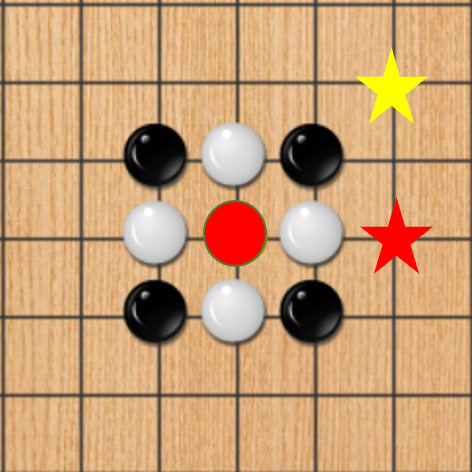
\includegraphics[scale=0.4]{example1.png}
    	\caption{An example of point update}
    	\label{figure}
    \end{figure}
    In Figure 2, we can see if we assume that the red dot is a black piece, then when we place another black piece at the position of the red five-pointed star, the value of the red dot will not change, and place a black piece at the position of the yellow five-pointed star, then its value Will change from 2000 to 200000. For the situation on the picture, placing any black piece in the horizontal and vertical directions of the red dot will not affect its score, because it is blocked from the influence of the other pieces in these two directions. So during a update process of a black piece, when AI meets a white piece, it just skip this direction, vice versa.
    \subsection{Zobrist hash}
    When scoring each checkerboard state, it takes a considerable amount of time to go through each grid point, and the same state can be reached through different sequences of choices, which cause time-consuming unnecessary duplicate searches. We can use the Zobrist hashing method to record the borad state with it's related information in order to avoid duplicate evaluations.
    \begin{figure}[H]
    \centering
    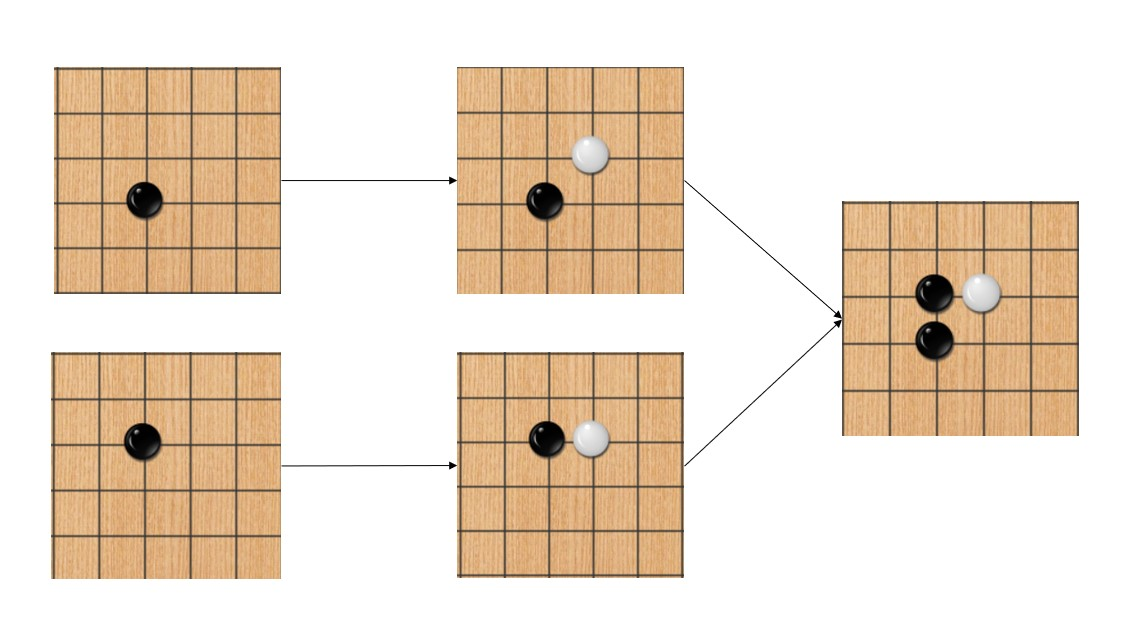
\includegraphics[scale=0.25]{figure1.jpg}
    \caption{An example of reaching the same state}
    \label{figure}
    \end{figure}
    Zobrist hashing, named after its inventor Albert L.Zobrist, is an encoding method specifically designed for board games. Zobrist hashes encode the checkerboard on an integer with a very low collision rate by using a special permutation table that assigns a coded index value to each possible state at each position on the board.
    
    It's implemented as follows, first generating a random number in the range of 64-bit integers for the black and white states at each point on the (15*15) board. For a specific board state, the random number corresponding to the color states at each point is XOR operation, and the result is the hash value. Whenever a node is searched, we store the result in the hash table with the Zobrist value as its key, and when a node is searched, we try to retrieve it's information from the table to use it.
    
    Zobrist is so efficient that only one XOR is required for each move, and the performance cost of this XOR is negligible compared to the score of each move. However, because each board state exists in the score\_graph, it iterates over its own submethods when updating the board. This causes the value in the hash table to be the score\_graph object which is deep-copied.
    
	After analysis, we believe that the efficiency of deep copies in python is not high enough and the board state of Gomoku is not complex enough, resulting the efficiency improved by it compared to the time spent on storage is not cost-effective. So we didn't use it in the end, but we still provides the interface to turn it on.


    \subsection{Threat Space With The Essential Move}
    In Gomoku, a threat is an important notion. According to the previous pattern definition, BLOCK\_FOUR and THREE can be considered as a threat. According to Victor Allis's theory, to win the game against any opposition a player needs to create a double threat. During a real backgammon game, there are often some moves that need no extra thought, because if we don't take those certain actions, we will lose directly or miss the chance to win.
    \begin{figure}[H]
    \centering
    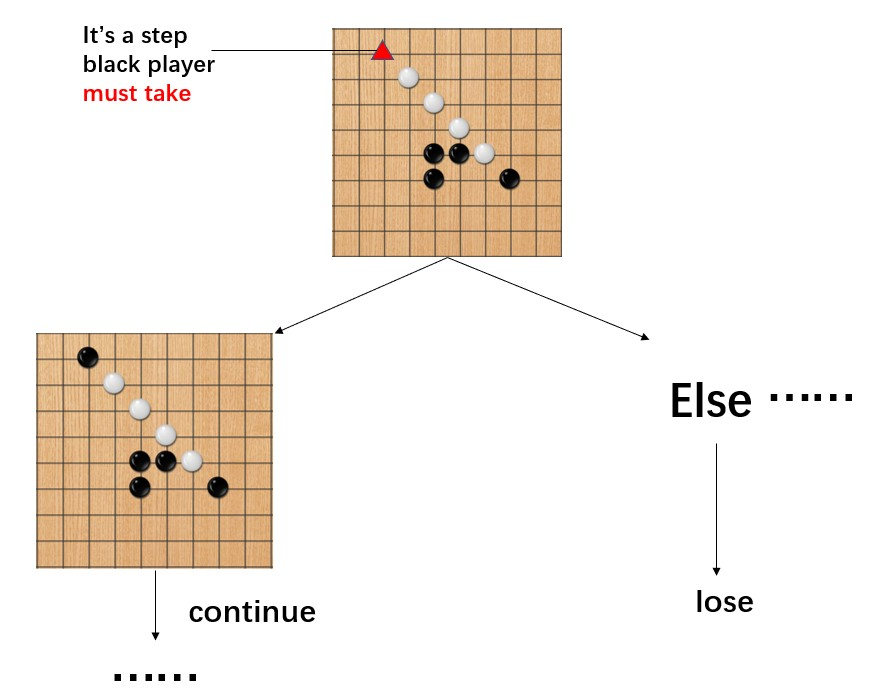
\includegraphics[scale=0.45]{figure2.jpg}
    \caption{An example of a step that player must take}
    \label{figure}
    \end{figure}
    By shifting the thinking mode of human to the modular program, we can create a function focus on searching in the threat space. Notably, the size of the search space is considerably reduced by first searching for the attacker's side. Thus, we creat a function called seek\_must, whose basic algorithm is as follows.
    \begin{algorithm}[H]
		\caption{seek essential point}
		\begin{algorithmic}[2]
			\Ensure value, action
			\If{we have win point}
        \State make that move to win
      \Else
        \If {opponent has win point}
          \State we should take it
        \Else
          \If {we have patterns of the THREE}
            \State we make that move
          \Else
            \If{opponent has patterns of the THREE}
              \State we should defuse the threat
            \EndIf
          \EndIf
        \EndIf
      \EndIf
    \end{algorithmic}
	  \end{algorithm}

    \subsection{Check Kill}
    Kill steps refer to a method that a player through the continuous THREE and BLOCK\_FOUR to attack, until the win. We tend to divide kill steps into two categories. One is VCF (Victory of Continuous BLOCK\_FOUR), and the other is VCT (Victory of Continuous THREE).
    
	In general, when calculating the kill steps, after making sure both sides do not have a point that leads to win, we carry out VCT first and then carry out VCF when no results are found before. Obviously, with the same depth and frame, the calculation is much more efficient than the previous search. Because in the case of checking kill, each node only counts the children of THREE and BLOCK\_FOUR. 
	
	Because of the high efficiency of checking kill, we can use more time to calculate at very large depth. To avoid overtimeing, we set a maximum running time for it and keep checking for timeouts. This will moderately increase the game power of the AI.


\end{multicols}

%----------------------------------------------------------------------------------------
\begin{multicols}{2}
  [
      \section{Experimental results}
  ]
    \begin{figure}[H]
    \centering
    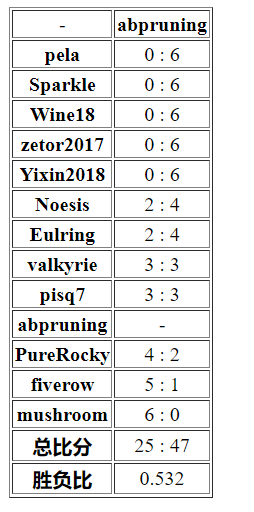
\includegraphics[scale=0.45]{result.png}
    \caption{experiment result}
    \label{figure}
    \end{figure}
  	The experimental results against other AIs can be found in Table 2. Our AI has been able to beat MUSHROOM completely, and beat PUREROCKY, FIVEROW by a large margin. Also, it's almost as strong as EULRING, VALKYRIE, PISQ7 and NOESIS. However, compared with other AIs, there is still a certain gap, which suggests that we should continue to improve it through future work.
  
 	For the sake of time limit, currently our parameters are determined based on the goal of making a move within 5 seconds. And in order to ensure better robustness, the parameters were set very conservatively. Now every time a decision is made, a  8-deep-level abp search is performed, and the branching factor is decreased to [8, 8, 8, 4, 4, 4, 4, 4, 4], and then the Check Kill module is used to do 8-deep-level search starting from the leaf node. We firmly believe the parameter performance still can be further improved.

\end{multicols}
%----------------------------------------------------------------------------------------

\begin{multicols}{2}
  [
      \section{Future Work}
  ]
  \subsection{Activemove Update Optimization}
  We can optimize the update process of the Activemove list, since each state change of the board only involves one point position. In this way, when we are looking for effective Activemove��s candidate points, we only need to delete the new point in the original list and add the expanded points around the new point, instead of going through the board and searching again.
  
  \subsection{Proof Number Search}
  Proof number search selects the next node to be expanded using two criteria: the potential range of subtree values and the number of nodes which must conspire to prove or disprove that range of potential values. These two criteria enable pn-search to treat efficiently game trees with a non-uniform branching factor.
  
  It is shown that in non-uniform trees proof number search outperforms other types of search, such as alpha-beta iterative-deepening search, even when enhanced with transposition tables. Thus, we plan to use pn-search to make check kill module more efficient.
  
\end{multicols}

%----------------------------------------------------------------------------------------
\begin{thebibliography}{99}  

  	\bibitem{ref1}L. Allis, H. Herik, and M. Huntjens. Go-moku and
	threat-space search. Computational Intelligence, 12, 10 1994.
  	\bibitem{ref2}Pearl, Judea. "The solution for the branching factor of the alpha-beta pruning algorithm and its optimality." Communications of the ACM 25.8 (1982): 559-564.
 	\bibitem{ref4}Albert Zobrist (1970). A New Hashing Method with Application for Game Playing. Technical Report, Computer Science Department, The University of Wisconsin, Madison, WI, USA.
  	\bibitem{ref3}J. Lawrence Carter, Mark N. Wegman (1977). Universal classes of hash functions. STOC'77

\end{thebibliography}


\bigskip
%----------------------------------------------------------------------------------------
%	REFERENCE LIST
%----------------------------------------------------------------------------------------

% \cite{Bird2014}
% \printbibliography

%----------------------------------------------------------------------------------------

\end{document}
